\documentclass{hrumc}

\usepackage{lipsum}
% \makeglossaries
\usepackage{makeidx}
\makeindex
\begin{document}
\newgeometry{left=1.25in,right=1.25in,bottom=1in,top=1in}
\onecolumn

% ----------------------------
% front cover
\vspace*{2ex plus 1fil}
\fronttitle{XXIII}
\vspace*{5ex plus 1fil}
\begin{frontgraphic}
  \put(0,-.25){\makebox[0em]{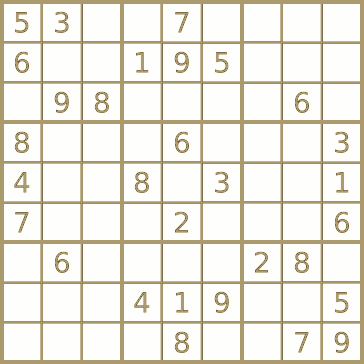
\includegraphics[scale=0.6]{sodoku.png}}}
  \put(0,-0.11){\makebox[0em]{
\includegraphics[scale=0.54]{pnp.png}}} % http://news.mit.edu/2009/explainer-pnp
\end{frontgraphic}
\vspace*{5ex}
\frontfoot
\vspace*{2ex plus 1fil}
\clearpage



% ----------------------------
% inside cover
\begin{scheduleoverview}
  8:30  &9:50am  &Registration             &Dion Center              \\
  10:00 &10:55am &Parallel Sessions One     &St~Edmunds and Jeanmarie Halls \\
  11:05 &12:15pm &Welcome, Invited Address  &McCarthy Arts Center     \\
  12:25 &1:30pm  &Lunch                     &Dion Center              \\
  1:40  &2:55pm  &Parallel Sessions Two     &St~Edmunds and Jeanmarie Halls \\
  3:00  &3:25pm  &Coffee and refereshments  &Dion Center  \\
  3:30  &4:25pm  &Parallel Sessions Three   &St~Edmunds and Jeanmarie Halls
\end{scheduleoverview}
\vspace{2ex plus 1 fill}
\wifi{SMC-Guest}{PurpleKnights}
\fullprogram{http://joshua.smcvt.edu/hrumc/hrumc2016short.pdf}{http://joshua.smcvt.edu/hrumc/hrumc2016full.pdf}
\vspace*{5ex}
\begin{help}
      \item[Medical, fire, or police]
       In an emergency call 911. 
       For non-emergency security or safety issues, call campus 
       security at 802-654-2911, or simply dial 2911 from any campus phone. 
       There is a campus phone in each classroom.

    \item[Classroom equipment]
      To help with computers or other equipment 
      there will be student assistants, wearing special tee-shirts, 
      in or near each classroom.
      You can also call (802)~654-2959, 
      or dial 2959 from the campus phone in each classroom.

    \item[Rest rooms]
      There are rest rooms on each floor of the academic buildings
      JEM and STE.
      There is a unisex rest room on the second floor of JEM,
      next to room~277.
\end{help}
\clearpage


% ----------------------------
% welcome page
{\setlength{\parskip}{1.5ex}
\setlength{\parindent}{0ex}
\welcome{twenty third}{Westfield State College}

\vspace{2ex plus 1fil}
\support{This conference would not be possible without the generous 
financial 
support provided by the Office of the Vice President for Academic Affairs 
at Saint Michael's College, and by the Departments of Mathematics and
Computer Science.
Support also comes from the NASA-VT Space Grant Consortium,
and from the Pi Mu Epsilon national mathematics honor society.}

\vspace{2ex plus 1fil}
\begin{minipage}{\textwidth}
  \begin{hrumcsteering}
  Lauren Childs, Williams College        \\
  Paul Friedman, Union College           \\
  Mohammad Javaheri, Siena College       \\
  Emelie Kenney, Siena College           \\
  Joe Kirtland, Marist College           \\
  Allison Pacelli, Williams College      \\
  Alejandro Sarria, Williams College     \\
  David Vella, Skidmore College          \\
  William Zwicker, Union College
  \end{hrumcsteering}
  \hspace{5em plus 1fill}
  \begin{localsteering}
  Jim Hef{}feron \\
  Lloyd Simons  
  \end{localsteering}
\end{minipage}
}
\clearpage


% ----------------------------
% plenary address page
\plenaryhead{Dr.~Karen Talentino, VPAA, Saint Michael's College}{Celsey Lumbra, SMC '16}
\vspace*{5ex}
\begin{plenary}{The $\mathbf{P}$ vs.\ $\mathbf{NP}$ Problem}{Scott Aaronson}{MIT, University of Texas at Austin}{Professor Aaronson 
holds a Ph.D.\ in Computer Science from University of California, Berkeley.
He is currently Associate Professor of Electrical Engineering and 
Computer Science
at the Massachussets Institute of Technology. 
Starting in July he will be the 
David J.~Bruton Jr.\ Centennial Professor of Computer Science at the 
University of Texas at Austin. 
He has an international reputation as an expert in the Theory of Computation 
and Complexity Theory.

Scott studies the fundamental limits on what can be efficiently computed in the physical world. This entails studying quantum computing, the most powerful model of computation that we have. His work has included limitations of quantum algorithms in the black-box model; the learnability of quantum states; quantum proofs and advice; the power of postselected quantum computing and quantum computing with closed timelike curves; and linear-optical quantum computing.}

I'll discuss the status of the famous 
$\mathbf{P}\mathbin{\hbox{?=}}\mathbf{NP}$ 
problem in 2016, offering
a personal perspective on what it's about, why it's important, why
many experts conjecture that $\mathbf{P}\mathbin{\hbox{!=}}\mathbf{NP}$ is both true and provable, why
proving $\mathbf{P}\mathbin{\hbox{!=}}\mathbf{NP}$ is so hard, the landscape of related problems, and
crucially, what progress has been made in the last half-century.  I'll
say something about diagonalization and circuit lower bounds; the
relativization, algebrization, and natural proofs barriers; and the
recent works of Ryan Williams and Ketan Mulmuley, which (in different
ways) hint at a duality between impossibility proofs and algorithms.
\end{plenary}
\vspace*{1ex plus 1fill}





% ===== BEGIN PARALLEL SESSIONS (leave this string; it is used by hrumc.py)


\sessionhead{One}
\session{Abstract Algebra I}{JEM 380}{Blair Madore}
\at{\Ia}{peterson} % 1  
\at{\Ib}{young} % 6
\at{\Ic}{mchugh} % 5

\session{Analysis}{JEM 389}{Andrew McIntyre}
\at{\Ia}{vees} % 9
\at{\Ib}{morfe} % 7
\at{\Ic}{jauregul} % 8

\session{Applied Mathematics Ia}{JEM 378}{Amy Wehe}
\at{\Ia}{phaneuf} % 26
\at{\Ib}{ratliff} % 12
\at{\Ic}{soper} % 13

\session{Applied Mathematics Ib}{JEM 166}{Eva Goedhart}
\at{\Ia}{desilva} % 22
\at{\Ib}{lerma} % 17
\at{\Ic}{vandermause} % 30

\session{Combinatorics I}{JEM 364}{Lauren Heller}
\at{\Ia}{kenney} % 38 
\at{\Ib}{boyadzhiyska} % 41 
\at{\Ic}{trenk} % 40

\session{Differential Equations I}{JEM 362}{To be announced}
\at{\Ia}{zachos} % 46
\at{\Ib}{bassette} % 51 
\at{\Ic}{mclaren} % 52

\session{Geometry I}{JEM 281}{Joseph Kirtland}
\at{\Ia}{ramrath} % 58
\at{\Ib}{johnson} % 57
% \at{\Ic}{martinez1} % 60

\session{Linear Algebra}{JEM 377}{William Zwicker}
\at{\IIIa}{warzer} % 77
\at{\IIIb}{ogle} % 76
\at{\IIIc}{reams} % 75

\session{Number Theory I}{JEM 168}{Paul Friedman}
\at{\Ia}{jia} % 91
\at{\Ib}{isham} % 86 
\at{\Ic}{chong} % 92

\session{Paradoxes}{JEM 375}{Daniel Velleman}
\at{\Ia}{harding} % 28
\at{\Ib}{daniere} % 117
\at{\Ic}{quenell} % 39

\session{Statistics Ia}{STE 104}{Phil Yates}
\at{\Ia}{schuckers} % 100 
\at{\Ib}{west} % 96
\at{\Ic}{trono} % 112

\session{Statistics Ib}{STE 102}{Jessica Mao}
\at{\Ia}{okeeffe} % 109
\at{\Ib}{pan} % 113
\at{\Ic}{roque} % 25

\session{Topology}{JEM 373}{Adam Lowrance}
\at{\Ia}{daley} % 115
\at{\Ib}{gall} % 116
\at{\Ic}{dragon} % 118






\sessionhead{Two}

\session{Abstract Algebra II}{JEM 373}{John McHugh}
\at{\IIa}{mchugh} % 2
\at{\IIb}{dever} % 4
\at{\IIc}{gibson} % 62

\session{Applied Math IIa}{JEM 378}{Ellen Gasparovic}
\at{\IIa}{ryzin} % 11
\at{\IIb}{hodge} % 20
\at{\IIc}{westland1} %10
\at{\IId}{afinogenov} % 94

\session{Applied Math IIb}{JEM 166}{Jeff Jauregui}
\at{\IIa}{kramer} % 23
\at{\IIb}{vrimoet} % 24
\at{\IIc}{holmes} % 27
\at{\IId}{kadas} % 15

\session{Combinatorics II}{JEM 364}{David Vella}
\at{\IIa}{vella} % 36
\at{\IIb}{bryant} % 31
\at{\IIc}{lane} % 32
\at{\IId}{halden} % 33

\session{Computer Science}{JEM 389}{William Dundar}
\at{\IIa}{zwicker} % 45
\at{\IIb}{claassen} % 42
\at{\IIc}{orzell} % 43
\at{\IId}{barrett} % 44

\session{Differential Equations II}{JEM 362}{Jenna Reis}
\at{\IIb}{klein} % 49
\at{\IIa}{buck} % 47
\at{\IIc}{li} % 54
% \at{\IId}{}

\session{Geometry II}{JEM 281}{Ockle Johnson}
\at{\IIa}{bania} % 63 
\at{\IIb}{hulbregtse} % 59
\at{\IIc}{ferlini} % 61

\session{Graph Theory}{JEM 380}{Adam Lowrance}
\at{\IIa}{holbrooks} % 66
\at{\IIb}{howard} % 67
\at{\IIc}{tremblay} % 65
\at{\IId}{whelan} % 64

\session{Graph Theory and Topology}{JEM 377}{Andrew McIntyre}
\at{\IIa}{luangrath} % 68 
\at{\IIb}{mcintyre} % 119
\at{\IIc}{chernov} % 114
% \at{\IId}{} %

\session{Mathematics Education I}{JEM 168}{Li-Mei Lim}
\at{\IIa}{raymond} % 79 
\at{\IIb}{bouchard} % 82
\at{\IIc}{tironi} % 81
\at{\IId}{czupryna} % 83

\session{Number Theory II}{JEM 375}{John Trono}
\at{\IIa}{paight} % 87 
\at{\IIb}{landfair} % 88
\at{\IIc}{northshield} % 89
\at{\IId}{ratliff1} % 93

\session{Statistics IIa}{STE 104}{Philip Yates}
\at{\IIa}{escobar} % 101
\at{\IIb}{hurlbut} % 102
\at{\IIc}{amerman} % 104
\at{\IId}{martinez} % 108

\session{Statistics IIb}{STE 102}{Amy Wehe}
\at{\IIa}{darrow} % 99
\at{\IIb}{markiewicz} % 106
\at{\IIc}{cameron} % 111
\at{\IId}{mcgraw} % 103






\sessionhead{Three}

\session{Applied Math IIIa}{STE 102}{Jeff Jauregui}
\at{\IIIa}{field} % 19
\at{\IIIb}{curtin} % 18
\at{\IIIc}{turner} % 14

\session{Applied Math IIIb}{JEM 378}{John McHugh}
\at{\IIIa}{wood} % 16
\at{\IIIb}{johnston} % 21
% \at{\IIIc}{}

\session{Combinatorics III}{JEM 362}{William Zwicker}
\at{\IIIa}{barde}  % 34
\at{\IIIb}{armstrong}  % 35
\at{\IIIc}{hernandez} % 37

\session{Differential Equations III}{JEM 166}{Zsuzsanna Kádas}
\at{\IIIa}{lefevre} % 48
\at{\IIIb}{oitsik} % 50
\at{\IIIc}{bennett} % 53

\session{Fractals and Chaos}{JEM 377}{Daniel M.\ Look}
\at{\IIIa}{healy} % 55
\at{\IIIb}{ostby} % 56
% \at{\IIIc}{}

\session{History of Mathematics}{JEM 281}{Paul Friedman}
\at{\IIIa}{hemingway} % 71
\at{\IIIb}{marinoff} % 69
\at{\IIIc}{gingrich} % 70

\session{Knot Theory}{JEM 389}{Richard Bedient}
\at{\IIIa}{lowrance} % 74
\at{\IIIb}{bennett} % 73
\at{\IIIc}{westland} % 72

\session{Mathematics Education II}{JEM 375}{George Ashline}
\at{\IIIa}{blue} % 78
\at{\IIIb}{stevens} % 80
\at{\IIIc}{ashline}

\session{Number Theory III}{JEM 364}{Blair Madore}
\at{\IIIa}{wyler} % 85
\at{\IIIb}{covey} % 90
\at{\IIIc}{nasser} % 84

\session{Probability and Statistics}{JEM 168}{Ada Morse}
\at{\IIIa}{bianco} % 95
\at{\IIIb}{mao} % 107
\at{\IIIc}{fredericks} % 105

\session{Statistics III}{STE 104}{Joseph Kirtland}
\at{\IIIa}{qi} % 98 
\at{\IIIb}{liu} % 97
\at{\IIIc}{davis} % 110

\session{Tropical Mathematics}{JEM 380}{Thomas Ratliff}
\at{\IIIa}{cheverie} % 3
\at{\IIIb}{hamelin} % 29
\at{\IIIc}{lee} % boris



% ===== END PARALLEL SESSIONS (leave this string; it is used by hrumc.py)

% Author index?
\ifbool{PrintAbstracts}{\printindex}{\relax}



% Back page is a campus map
\clearpage
\vspace*{0ex plus 1 fill}
\begin{map}[map.png]\large
    \begin{picture}(7.681,8.194)  % map is 7.681 by 8.194 inches
      \put(0,0){\usebox{\mapbox}}
      \put(-.2,1.4){\mapkey{1}{I-89 Exit 15 is a quarter mile this way}}
      \put(-.2,1.05){\mapkey{2}{Enter here, park on your left}}
      \put(-.2,.7){\mapkey{3}{McCarthy Arts building; invited address}}
      \put(-.2,.35){\mapkey{4}{Saint Edmunds Hall (STE); parallel sessions}}
      \put(-.2,.0){\mapkey{5}{Jeanmarie Hall (JEM); parallel sessions}}
      \put(-.2,-0.35){\mapkey{6}{Dion Center; register, lunch, and break}}
      \put(-.2,-0.7){\parking\hspace{0.75em}Parking}
      \put(1,8){\circled{1}}
      \put(1.6,5.3){\circled{2}}
      \put(2.6,4.8){\circled{3}}
      \put(2.55,3.7){\circled{4}}
      \put(1.56,3.7){\circled{5}}
      \put(4,3.5){\circled{6}}
      \put(1.77,5.63){\parking}
      \put(2.3,5.63){\parking}
      \put(1.95,6.4){\parking}
      \put(1.95,7.1){\parking}
      \put(1.8,7.75){\parking}
    \end{picture}   
\end{map}
\vspace*{0ex plus 1fill}

\end{document}
